\documentclass[a4paper,10pt]{report}
\usepackage{cours}
\usepackage{tkz-tab}
\usepackage[dvipsnames]{xcolor}
\usepackage{textcomp, fancyvrb,multicol}
\usepackage{tkz-tab}
\usepackage[dvipsnames]{xcolor}
\begin{document}
\everymath{\displaystyle}


\begin{center}
\textit{{ {\huge TD 7 : Fonctions vectorielles et arc param�tr�s}}}
\end{center}


\medskip

%\noindent $I$ d�signe un intervalle de $\mathbb{R}$ contenant au moins deux points et $n$ est un entier naturel non nul.
%
%\medskip

%
%
%\begin{center}
%{\large \textit{\underline{Fonctions vectorielles}}}
%\end{center}
%
%\medskip
%
%\exo Soit $f : I \rightarrow \R^n$ une fonction de classe ${\cal C}^1$ sur $I$.  On suppose que l'application $\|f\|$ est constante. Montrer que pour tout $t\in I,$ $f(t)\perp f'(t).$
%
%\exo Soient $a$, $b$, $c$ et $d$, des fonctions d�rivables sur $I$. Donner de deux mani�res la d�riv�e de la fonction $f$ d�finie par :
%$$ f(x)  = \left\vert \begin{array}{cc}
%a(x) 	& b(x) \\
%c(x) & d(x) \\
%\end{array}\right\vert$$
%
%\exo Soit $f : ]-1,1[ \rightarrow \mathbb{R}^2$ d�fini par :
%$$ f(t) = \left\lbrace \begin{array}{cl}
%(0,0) & \hbox{ si } t \in ]-1,0] \\
%\left( t^2  \cos \left( \dfrac{1}{t} \right), t^2  \sin \left( \dfrac{1}{t} \right) \right) & \hbox{ si } t \in ]0,1[ \\
%\end{array}\right.$$
%Montrer que $f$ est d�rivable sur $]-1,1[$ et donner $f'$.
%
%
%
%\begin{center}
%{\large \textit{\underline{Arcs param�tr�s}}}
%\end{center}
%
%\medskip

\begin{Exa} �tudier l'arc param�tr� du plan d�fini par :
$$ x(t) = t^2+ \dfrac{2}{t}, \; y(t) = t^2+\dfrac{1}{t^2} $$
\end{Exa}

\corr Posons $f=(x,y)$. La fonction $f$ est d�finie sur $\mathbb{R}^*$. L'ensemble d'�tude est aussi $\mathbb{R}^*$ (pas de p�riodicit�, $y$ est paire mais $x$ n'est ni paire ni impaire).

\medskip

\noindent La fonction $f$ est de classe $\mathcal{C}^1$ sur $\mathbb{R}^*$ et pour tout $t \in \mathbb{R}^*$,
$$ x'(t) = 2t - \dfrac{2}{t^2} = 2 \times \dfrac{t^3-1}{t^2}$$
et
$$ y'(t) = 2t -\dfrac{2}{t^3} = 2 \times \dfrac{t^4-1}{t^3} = 2 \times \dfrac{(t^2-1)(t^2+1)}{t^3}$$
Remarquons que $x'(t)$ et de signe de $t^3-1$ donc positif si et seulement si $t \geq 1$. Le signe de $y'(t)$ est celui de :
$$ \dfrac{t^2-1}{t^3}$$
qui est facile � obtenir. On obtient le tableau de variations suivant (apr�s calculs des limites) :

\begin{center}
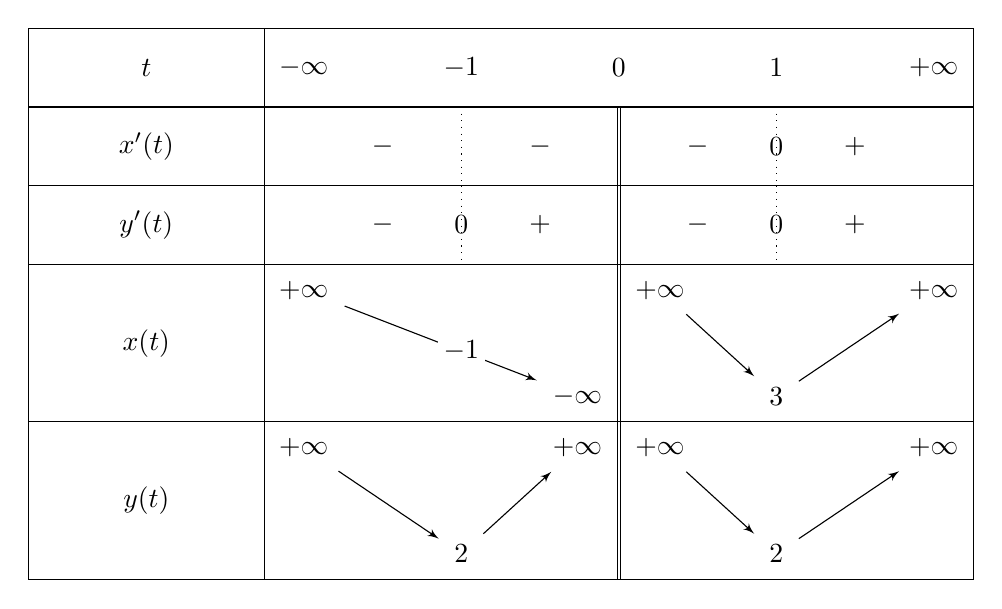
\begin{tikzpicture}
   \tkzTabInit[lgt = 3,espcl =2]{$t$ / 1 , $x'(t)$ / 1, $y'(t)$ /1,$x(t)$/2,$y(t)$/2}{$-\infty$, $-1$, $0$, $1$, $+\infty$}
   \tkzTabLine{, - , t , - , d , - , z,  + ,  }
   \tkzTabLine{, - , z , + , d , - , z,  + ,  }
   \tkzTabVar{+/ $+\infty$ , R/,-D+/$- \infty$/  $+\infty$ , -/$3$,+/ $+ \infty$} 
   \tkzTabIma{1}{3}{2}{$-1$}
   \tkzTabVar{+/ $+\infty$,-/$2$,+D+/$+ \infty$/$+\infty$,-/$2$,+/$+ \infty$ } 
\end{tikzpicture}
\end{center}
Le seul point singulier est le point de param�tre $1$. Pour tout $t \in \mathbb{R}$, posons $u=t-1$ (ce qui implique que $t=u+1$). Alors $t$ tend vers $1$ si et seulement si $u$ tend vers $0$ ce qui permet d'obtenir les d�veloppements limit�s suivants quand $t$ tend vers $1$ :
\begin{align*}
x(t) &= x(1+u)  \\
& = (1+u)^2 + \dfrac{2}{1+u} \\
&  \underset{u \rightarrow 0}{=} 1+2u+u^2 +2(1-u+u^2-u^3+o(u^3)) \\
& \underset{u \rightarrow 0}{=} 3+3u^2-2u^3+o(u^3) \\
&  \underset{t \rightarrow 1}{=} 3 + 3(t-1)^2-2(t-1)^3 + o ((t-1)^3) 
\end{align*}
et 
\begin{align*}
y(t) & = y(1+u) \\
& = (1+u)^2 + \dfrac{1}{(1+u)^2} \\
& \underset{u \rightarrow 0}{=} 1+2u+u^2 + (1-u+u^2-u^3+o(u^3))^2 \\
&  \underset{u \rightarrow 0}{=} 1+2u+u^2 + 1-u+u^2-u^3 -u+u^2-u^3+u^2-u^3-u^3+o(u^3) \\
& \underset{u \rightarrow 0}{=} 2+4u^2-4u^3+o(u^3) \\
& \underset{t \rightarrow 1}{=} 2+4(t-1)^2-4(t-1)^3+o((t-1)^3)
\end{align*}
Les vecteurs $(3,4)$ et $(-2,-4)$ sont non colin�aires donc on pose $(p,q)=(2,3)$. Ainsi, le point de param�tre $1$ est un point de rebroussement de premier esp�ce.

\medskip

\noindent �tudions maintenant les branches infinies. On a :
$$ \dfrac{y(t)}{x(t)}  \underset{+ \infty}{\sim} \dfrac{t^2}{t^2} = 1$$
et 
$$ y(t)-x(t) = \dfrac{1}{t^2}- \dfrac{2}{t} \underset{t \rightarrow + \infty}{\longrightarrow} 0$$
On obtient les m�mes calculs au voisinage de $- \infty$. Ainsi, la droite d'�quation $y=x$ est asymptote au support $\Gamma$ en $+ \infty$ et $- \infty$.

\medskip

\noindent On a : 

$$ \dfrac{y(t)}{x(t)}  \underset{0}{\sim} \dfrac{1/t^2}{2/t} = \dfrac{1}{2t}$$
donc 
$$ \lim_{t \rightarrow 0^+} \dfrac{1}{2t} = + \infty$$
et 
$$ \lim_{t \rightarrow 0^+} \dfrac{1}{2t} = - \infty$$
Ainsi, le support admet une branche parabolique de direction $(0y)$ en $0$.

\medskip

\noindent Voici une repr�sentation graphique obtenu avec Python. Sur une copie, il faudrait bien faire apparaitre la droite d'�quation $y=x$ et la tangente horizontale d'�quation $y= 2$ � $\Gamma$ au point de param�tre $-1$.

\medskip

\begin{center}
\includegraphics[scale=0.3]{ex1}
\end{center}

\medskip

\noindent Pour les curieux, le code :

\begin{verbatim}
import pylab as pl
import numpy as np


T=np.linspace(-5,5,51) # tableau des valeurs de t (on �vite la valeur 0)
def x(t) : 
    return t*t+2/t
def y(t) : 
    return  t*t+1/(t*t)

X=x(T) # tableau des abscisses 
Y=y(T) # tableau des ordonn�es

pl.axis('equal') # permet d'avoir un rep�re orthonorm�
pl.plot(X,Y) # trac� de la courbe
pl.show() # affichage du trac�
\end{verbatim}

\end{document}
